\documentclass[11pt]{article}
\usepackage[margin=0.85in]{geometry}
\usepackage{amsmath,amssymb,graphicx,xurl,hyperref}
\setlength{\parindent}{0pt}\setlength{\parskip}{7pt}
\begin{document}
{\LARGE Constructed finite rational Hermite recovery}\par
November9,2026. Mathematical source \texttt{bd8cbfe231702221685d3f99cfa91f6168cbb797}.
Unsigned producer evidence throughout [pcc:unverified].

\textbf{Result.} Two finite coefficient buffers determine each modular quotient
jet. The explicit Hermite sum is integral and returns the original contraction
modulo $2^p$. No caller-supplied reconstruction or quotient-congruence premise
remains. The algorithmic value is the constructed sum; the known target is used
only in its correctness proof.

\textbf{Domain.} Let $\mathcal O=\{r\in\mathbb Q:|r|_2\leq1\}$.
Assume $3\leq u\leq a$, $u\leq M$, injective supplied placement and integral
weights $A,B$. Put $L=2^a$, $\alpha=2L$, $h=\lceil3M/u\rceil$ and use the
actual centered nodes with orders $q(0)=0$ and
$q(t)=h\max(0,u-v_2(t))$. Output precision $p$ counts bits.

\textbf{Exact reconstruction.} Form
\[
 E_t(T)=\prod_{s\ne t}\left(\frac{T-s}{t-s}\right)^{q(s)},\qquad
 J_t(z)=\left[\frac{F(t+\alpha z)}{E_t(t+\alpha z)}\right]_{<q(t)}.
\]
Each summand $E_t(T)J_t((T-t)/\alpha)$ has the prescribed own-node jets and
vanishes to the required orders at other nodes. Its degree is below the total
multiplicity. Summation and exact uniqueness yield
\[
 F(T)=\sum_t E_t(T)J_t((T-t)/\alpha),\qquad
 F(0)=\sum_t E_t(0)J_t(-t/\alpha).
\]
The actual cleared contraction satisfies the required degree bound. Its local
integral chart maps exactly to this rational source chart.

\textbf{Finite construction.} Invert the length-$q(t)$ denominator vector with
constant coefficient one, convolve with the length-$q(t)$ input vector and
truncate. Mapping this finite operator to residues agrees with the exact
quotient coefficients. Canonical integer lifts give the actual input to the
recovery functional.
\newpage
{\Large Precision and dependency map}\par
Use the original source child precision
\[
 p_t=p+8hD_i+8M(a+1),\quad D_i=2^{a-i},\quad i=v_2(t).
\]
The previous component established actual multiplier loss $6hD_i$ and
local evaluation loss $4M(a+1)$. Thus the finite constructed coefficient
errors leave at least $p$ correct bits. The recovered sum lies in $\mathcal O$
and its image modulo $2^p$ equals that of $\sum_x A_xB_x$.

\begin{center}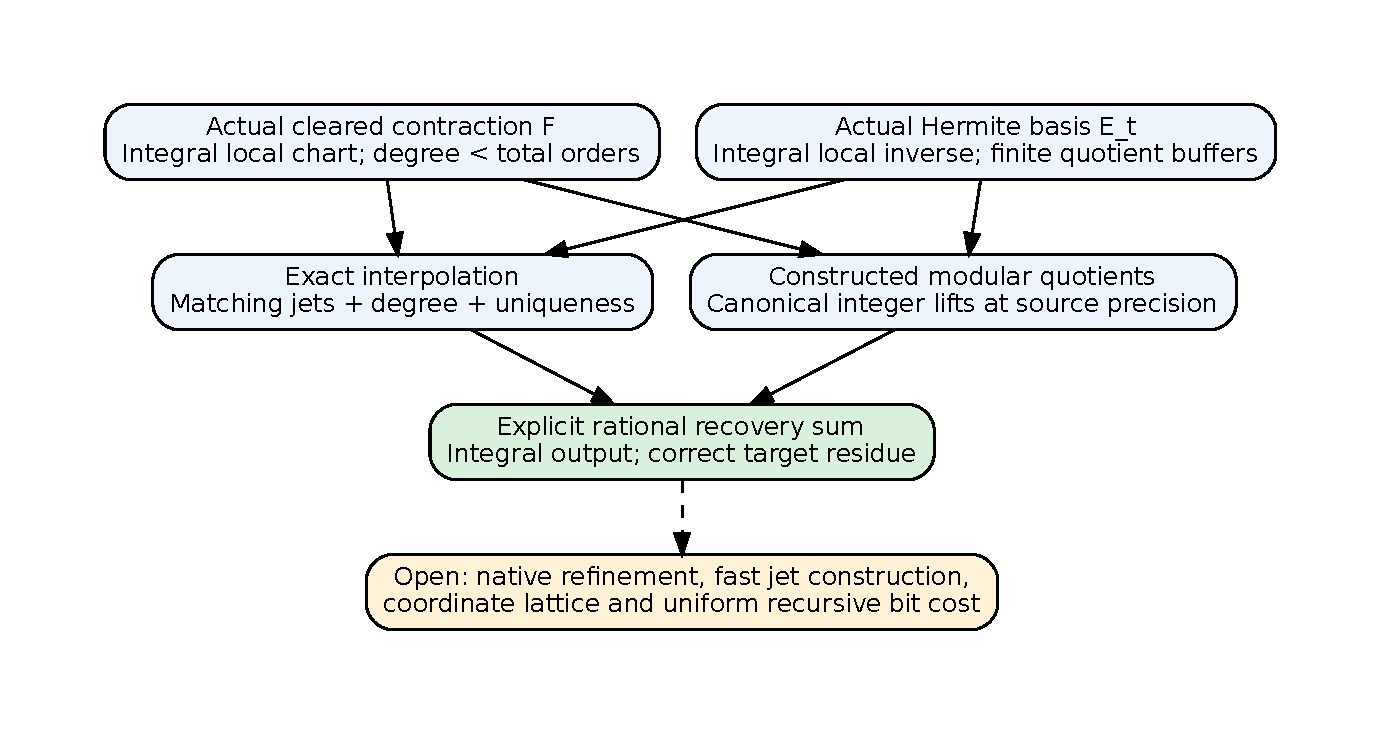
\includegraphics[width=0.9\linewidth,height=0.69\textheight,keepaspectratio]{bridge.pdf}\end{center}

The complete precision construction here is rational. The earlier exact
uniqueness statement over general $\mathbb Q$-algebras does not itself extend
this precision theorem to extension or nilpotent coefficient lattices.
\newpage
{\Large Evidence and continuation}\par
\textbf{Producer checks.} Default build:3198 completed jobs. Actual source
audit:269 declarations,0 additional trusted axioms. Import-inclusive
\texttt{leanchecker --fresh --verbose FiniteRecovery}: exit0.
Dependency axioms are restricted to propext, Classical.choice and Quot.sound.

Eight unsigned PCC records bind the declarations: exact reconstruction
(67badf), packed reconstruction (281660), exact evaluation (55e9c7), actual
integral chart (a4f1bb), quotient mapping (11770a), computed quotient residue
(33208a), computed recovery precision (e2bf84), computed target residue
(e57c3b). Prefix each suffix by \texttt{PCC-20261109-}.
Canonical declaration hashes and raw compressed build/replay logs are retained
under the study's \texttt{lean/} directory; failed attempts are included.

\textbf{Sources.} OpenAI, \emph{The Exponential Time Hypothesis is False},
October25,2026, D.4.2--D.4.4 and D.7--D.10, repository commit
\texttt{7ef5c0cc5ca4b0e072b7a050fca09ab24bc6fa3a}.
PDF SHA256: \nolinkurl{5b1612dc2eebb2cad5b4cbe62d1fed2982f01ab1908c26f70010a651487e8123}.
The preceding Hermite precision report and actual Lean declarations supply
the local context. KB unavailable; no novelty or exhaustive-search claim.

\textbf{Next discriminating test.} Implement native finite arithmetic and
freeze a separate bounded correctness census with defective controls and
identical replay before data collection. No timing data or measured gain is
reported in this phase. Earlier reports and frozen panel remain unchanged.

\textbf{Remaining proof obligations.} Native refinement, efficient construction
of input jets, coordinate precision maps and all-level recursive bit costs.
The finite formal-series specification alone gives no bound on their cost.
All statements retain unsigned producer standing pending signed verification.
\end{document}
